% Slides for 2024-10-21
% To create a slide, use the following:
% \begin{frame}{TITLE}
%     BODY
% \end{frame}

% To create a slide with a bullet list, use the following:
% \begin{frame}{TITLE}
%     \begin{itemize}
%         \item ITEM 1
%         \item ITEM 2
%     \end{itemize}    
% \end{frame}

% To create a slide with numbered list, use the following:
% \begin{frame}{TITLE}
%     \begin{enumerate}
%         \item ITEM 1
%         \item ITEM 2
%     \end{enumerate}
% \end{frame}

% To create a slide with a graphic:
% 1. Add the graphic to this folder (named picture.png)
% 2. Use the following:
% \begin{frame}{TITLE}
%     \centering
%     \includegraphics[height=0.7\textheight,width=0.7\textwidth,keepaspectratio]{picture.png}
% \end{frame}

% To create a slide with two columns, use the following:
% \begin{frame}{TITLE}
%     \begin{columns}
%         \begin{column}{0.5\textwidth}
%             COLUMN 1 BODY
%         \end{column}
%         \begin{column}{0.5\textwidth}
%             COLUMN 2 BODY
%         \end{column}
%     \end{columns}
% \end{frame}

\begin{frame}{Drone Ground Control Software}
    \begin{columns}
        \begin{column}{0.5\textwidth}
            \centering
            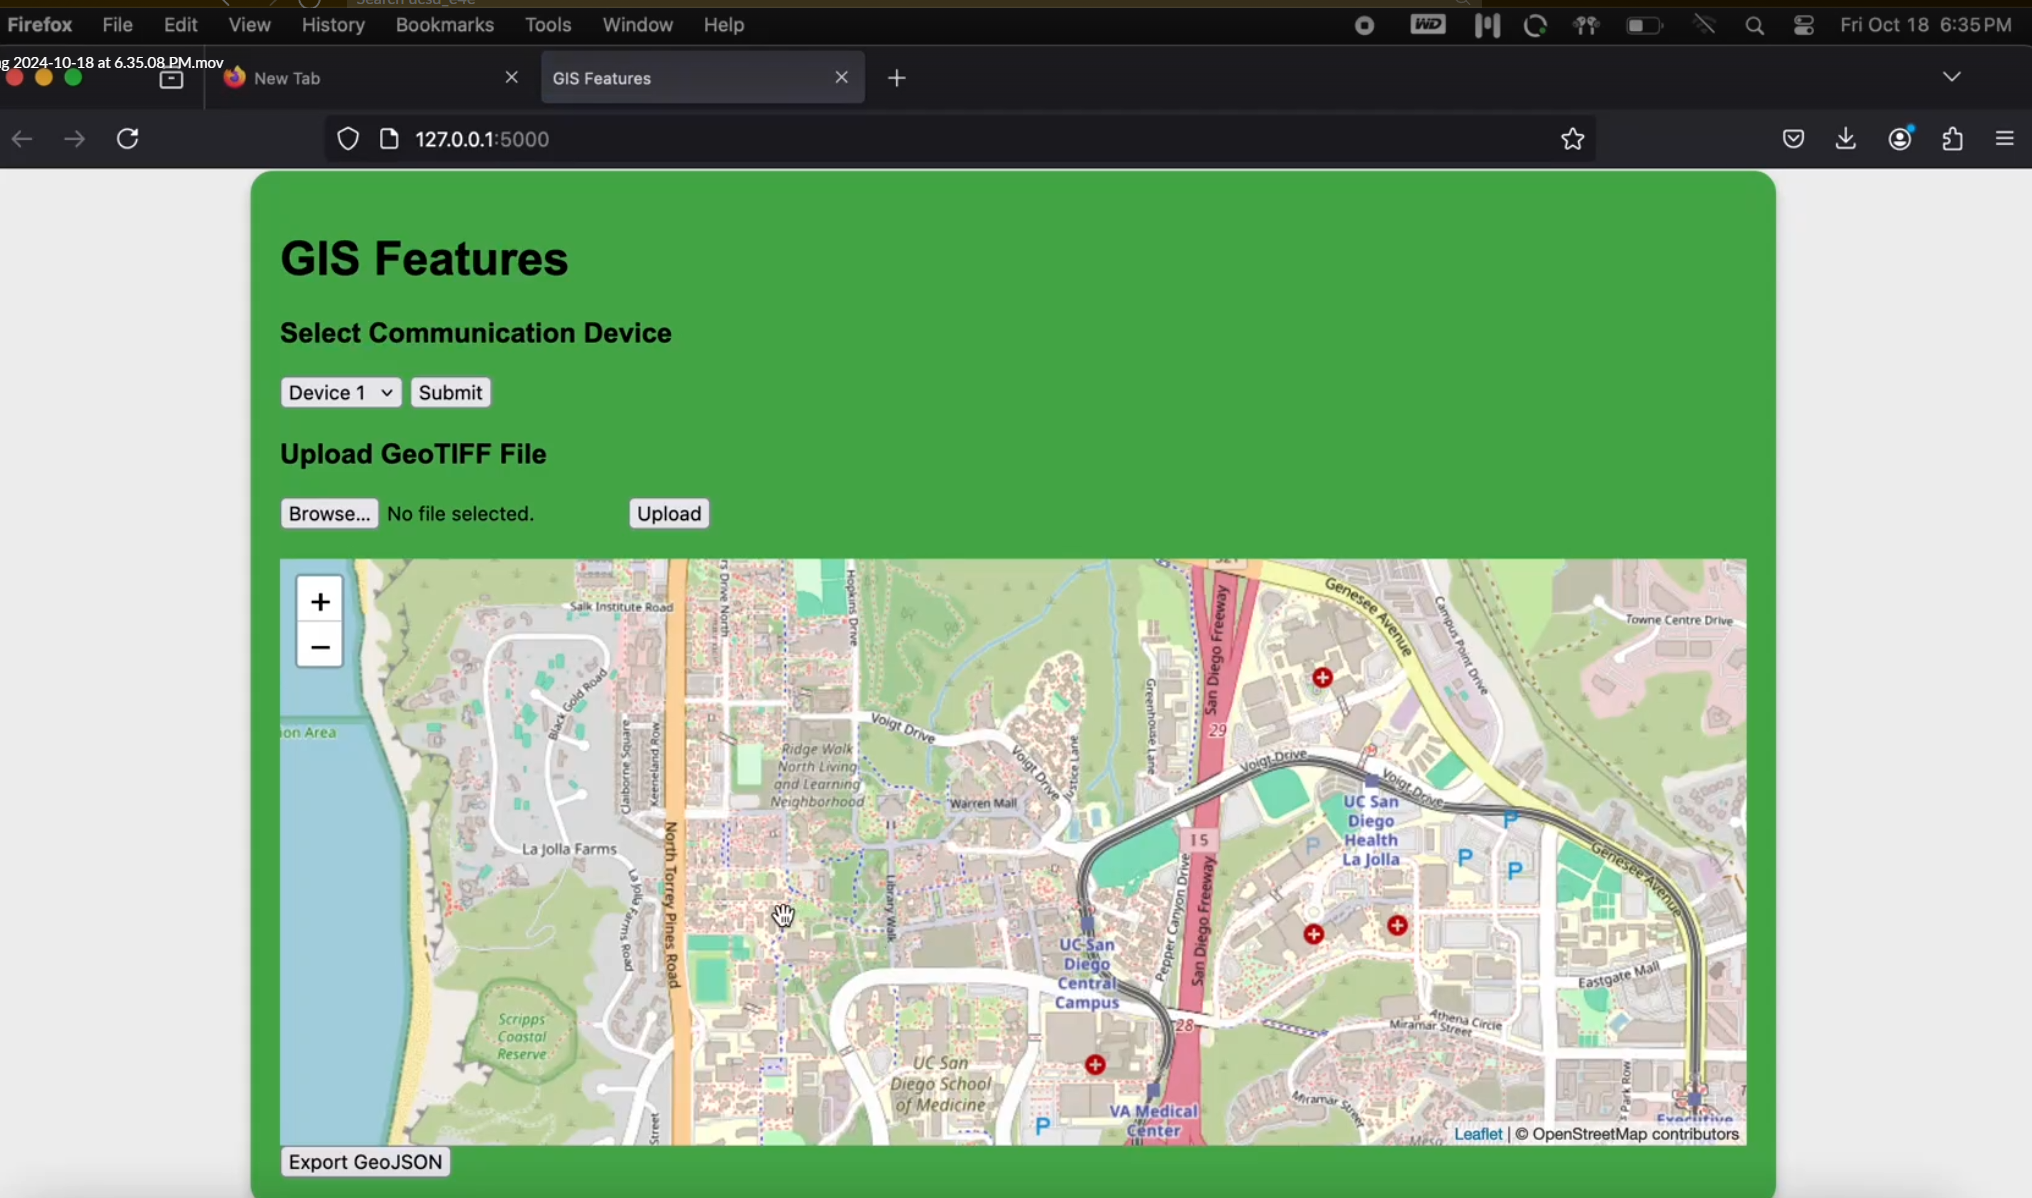
\includegraphics[height=0.7\textheight,width=\textwidth,keepaspectratio]{images/rtt/image.png}
        \end{column}
        \begin{column}{0.5\textwidth}
            \begin{itemize}
                \item Folium with leaflet.offline
                \begin{itemize}
                    \item GeoTIFF/GeoJSON/Shapefile support
                    \item OpenStreetMap support (offline with Overpass API)
                \end{itemize}
                \item Experimenting with GUI and devices
            \end{itemize}
        \end{column}
    \end{columns}
\end{frame}

\begin{frame}{Drone Field Device Software}
    \begin{tikzpicture}[remember picture,overlay]
        % Left image
        \node[anchor=north west,inner sep=50] at (current page.north west) {
            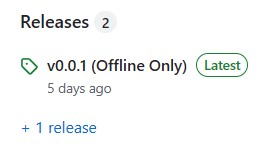
\includegraphics[height=\paperheight,width=0.4\paperwidth,keepaspectratio]{images/rtt/release.jpg}
        };
        % Right image
        \node[anchor=north east,inner sep=50] at (current page.north east) {
            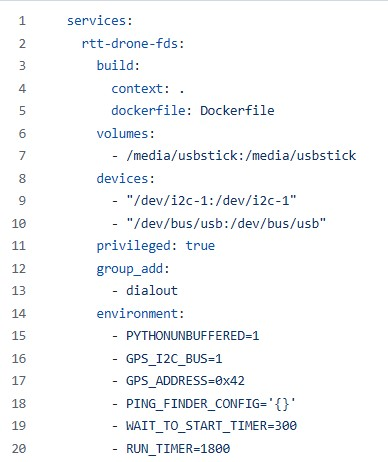
\includegraphics[height=\paperheight,width=0.4\paperwidth,keepaspectratio]{images/rtt/compose.jpg}
        };
        % Semi-transparent overlay for bullet points
        \fill[white,opacity=0.7] (current page.south west) rectangle ([yshift=2.5cm]current page.south west);
        % Bullet points
        \node[anchor=south west, text width=\paperwidth-1cm, inner sep=0.5cm] at (current page.south west) {
            \begin{itemize}
                \item No realtime tracker release made
                \item Some QOL improvements needed
                \item Field test ready but supporting items 
            \end{itemize}
        };
    \end{tikzpicture}
\end{frame}

\begin{frame}{Tower Hardware}
    \begin{columns}
        \begin{column}{0.5\textwidth}
            \centering
            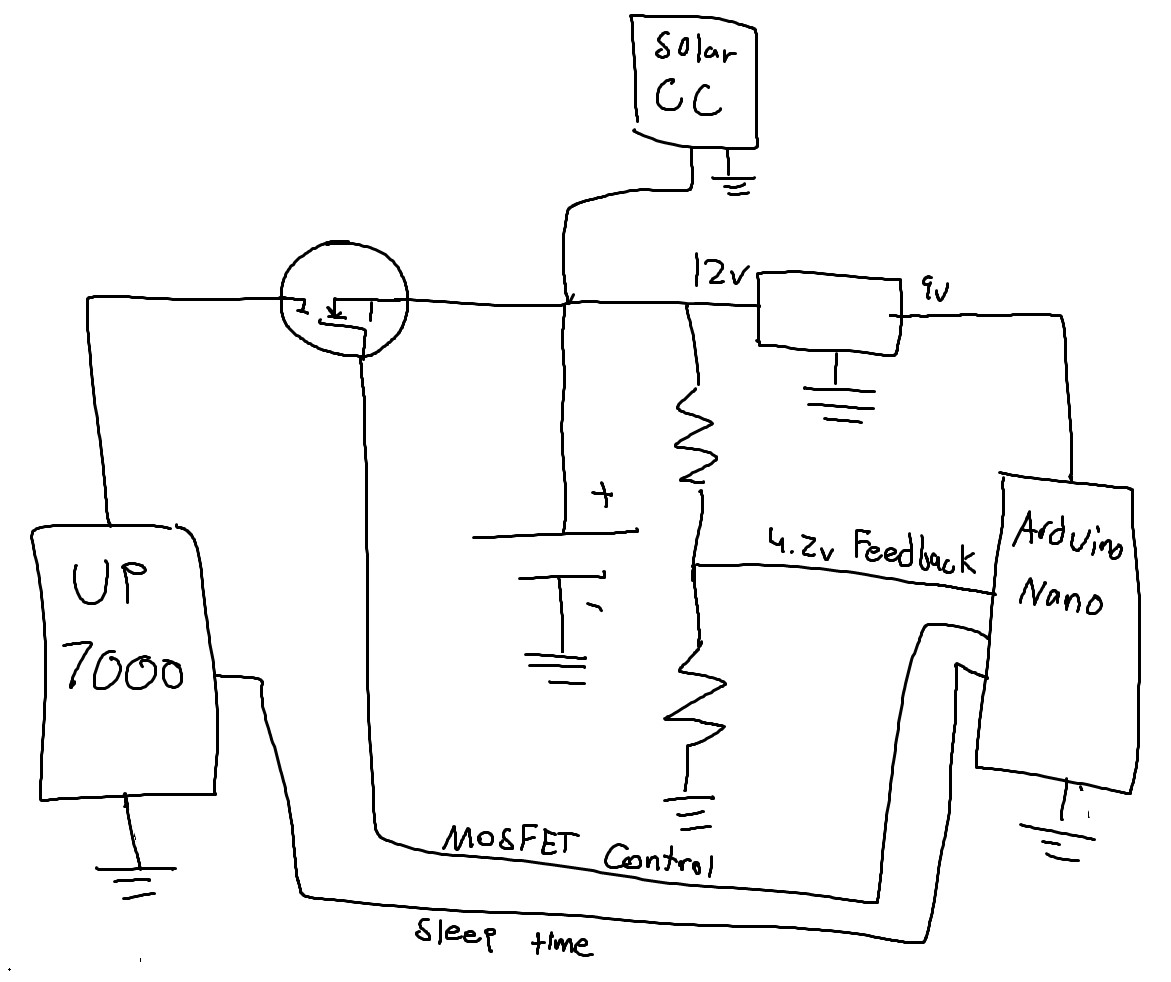
\includegraphics[height=0.7\textheight,width=\textwidth,keepaspectratio]{images/rtt/Screenshot 2024-10-21 013935.jpg}
        \end{column}
        \begin{column}{0.5\textwidth}
            \begin{itemize}
                \item Gathering parts list for sleep timer/solar power
                \item Much cheaper than initially estimated
            \end{itemize}
        \end{column}
    \end{columns}
\end{frame}
